\section{Chunk management system}\label{sec:chunk-worker}
The majority of the game logic is handled by a single thread.
The only two exceptions are the physics engine (external library) and the chunk management system.
The chunk management system is split between two threads: the main thread (the thread that the rest of the application is running on) and the \textit{chunk worker's} thread.
The worker's thread is concerned with operations that are either CPU-intensive or could take a long time to execute.
More specifically, the chunk worker is performing the following operations:
\begin{enumerate}
    \item loading saved chunks from disk and generating new chunks,
    \item saving chunks to disk,
    \item updating chunks.
\end{enumerate}
The system is built around the producer-consumer pattern, i.e. the main thread communicates with the worker's thread (and \textit{vice versa}) using queues.
It's important to note that depending on the stage of an operation either thread can be the \textit{producer} or the \textit{consumer}.
We will now describe the workflow for each of the operations mentioned before.

\subsection{Loading and generating chunks} \label{subsec:loading-and-generating}
On each render frame, the main thread calls the \texttt{UpdateCurrentPosition} method.
This method, based on the camera's current position and the render distance, determines which chunks should be loaded into the game.
If a chunk isn't already loaded or isn't queued for loading, the position of the chunk is enqueued into the \texttt{chunksToLoad} queue.

The worker thread in the \texttt{LoadChunks} function dequeues the positions of the chunks to be loaded from the disk.
If a chunk is not saved on the disk, it is generated.
The loaded/generated chunk is then enqueued into the \texttt{loaded} queue.

The main thread through the \texttt{ResolveLoaded} function dequeues a chunk and performs the following actions:
\begin{enumerate}
    \item creates a vertex array object for the chunk's mesh,
    \item creates a collision surface for the chunk,
    \item adds the chunk to the list of scene's chunks for rendering.
\end{enumerate}

It's worth noting that the operations in \texttt{ResolveLoaded} function have to be performed on the main thread because they interact with OpenGL and the physics engine APIs.
\subsection{Saving chunks}
Saving chunks is handled by a process similar to the one discussed in \autoref{subsec:loading-and-generating}.
On each frame, the main thread in the \texttt{DeleteChunks} function determines which chunks are too far from the player and thus should be removed from the game and saved to disk.
Positions of these chunks are enqueued into the \texttt{chunksToSave} queue, and their resources are freed.
More precisely, the removal takes place only if the number of chunks in the game exceeds a certain limit.
This is so that chunks are not deleted and loaded again constantly when the player moves back and forth between chunks.

The worker thread dequeues chunks' positions from the \texttt{chunksToSave} queue and saves the scalar field associated with a given chunk on the disk.
\subsection{Updating chunks}
Terrain modification consists of two main steps:
\begin{enumerate}
    \item the scalar field for the modified chunk has to be altered, which involves iterating over a 3-dimensional array of numbers and modifying the values stored in that array using some function,
    \item a new mesh has to be generated based on the new values of the scalar field.
\end{enumerate}
Since the modifications happen 60 times a second and the number of operations they require is rather big (of the order of the chunk size, i.e. $16^3$) it's unfeasible to do them on the main thread without severe lags.
Thus most of the work related to terrain modification is delegated to the worker thread.

The workflow for terrain modification can be described as follows.
The main thread in the \texttt{Pickaxe.ModifyTerrain} method determines which chunks are going to be affected by the terrain modification, and adds them to a buffer \texttt{buffer}.
Once all the chunks are in \texttt{buffer}, we set the \texttt{IsProcessingBatch} flag to \texttt{true} (while set to true, no further terrain modifications will be registered) and enqueue each of them into the \texttt{modificationsToPerform} queue along with some additional information (passed in the form of an instance of \texttt{ModificationArgs} struct) necessary to perform the modification.
A very important piece of information is the \texttt{batchSize} which is the size of \texttt{buffer} (its importance will become apparent later).

The worker thread dequeues chunks from the \texttt{modificationsToPerform} queue.
It modifies the scalar field using the information passed in \texttt{ModificationArgs} and generates a new mesh based on the scalar field.
Once new vertices for the mesh are calculated, it enqueues the chunk together with \texttt{batchSize} (retrieved from \texttt{modificationArgs}) into the \texttt{updatedChunks} queue.

In the \texttt{ResolveUpdated} function the main thread dequeues the \texttt{(chunk, batchSize)} pair from the \texttt{updatedChunks} queue and adds \texttt{chunk} to the \texttt{currentBatch} list.
Once the number of chunks in \texttt{currentBatch} is equal to \texttt{batchSize} of the dequeued chunk, it means that the main thread has "received back" all of the chunks from a single modification call.
The main thread then updates the GPU buffers with the new vertices of the chunk's mesh and updates the shape of the collision surface in the physics engine for each chunk from \texttt{currentBatch}.
Once the whole \texttt{currentBatch} is updated, the \texttt{IsProcessingBatch} flag is set back to false.

The whole process is depicted in \autoref{fig:chunk-worker}.
\begin{figure}[!htb] % https://drive.google.com/file/d/1TzJouYAys_fz1GkhppZsqoh9yFn62twL/view?usp=sharing
    \centering
    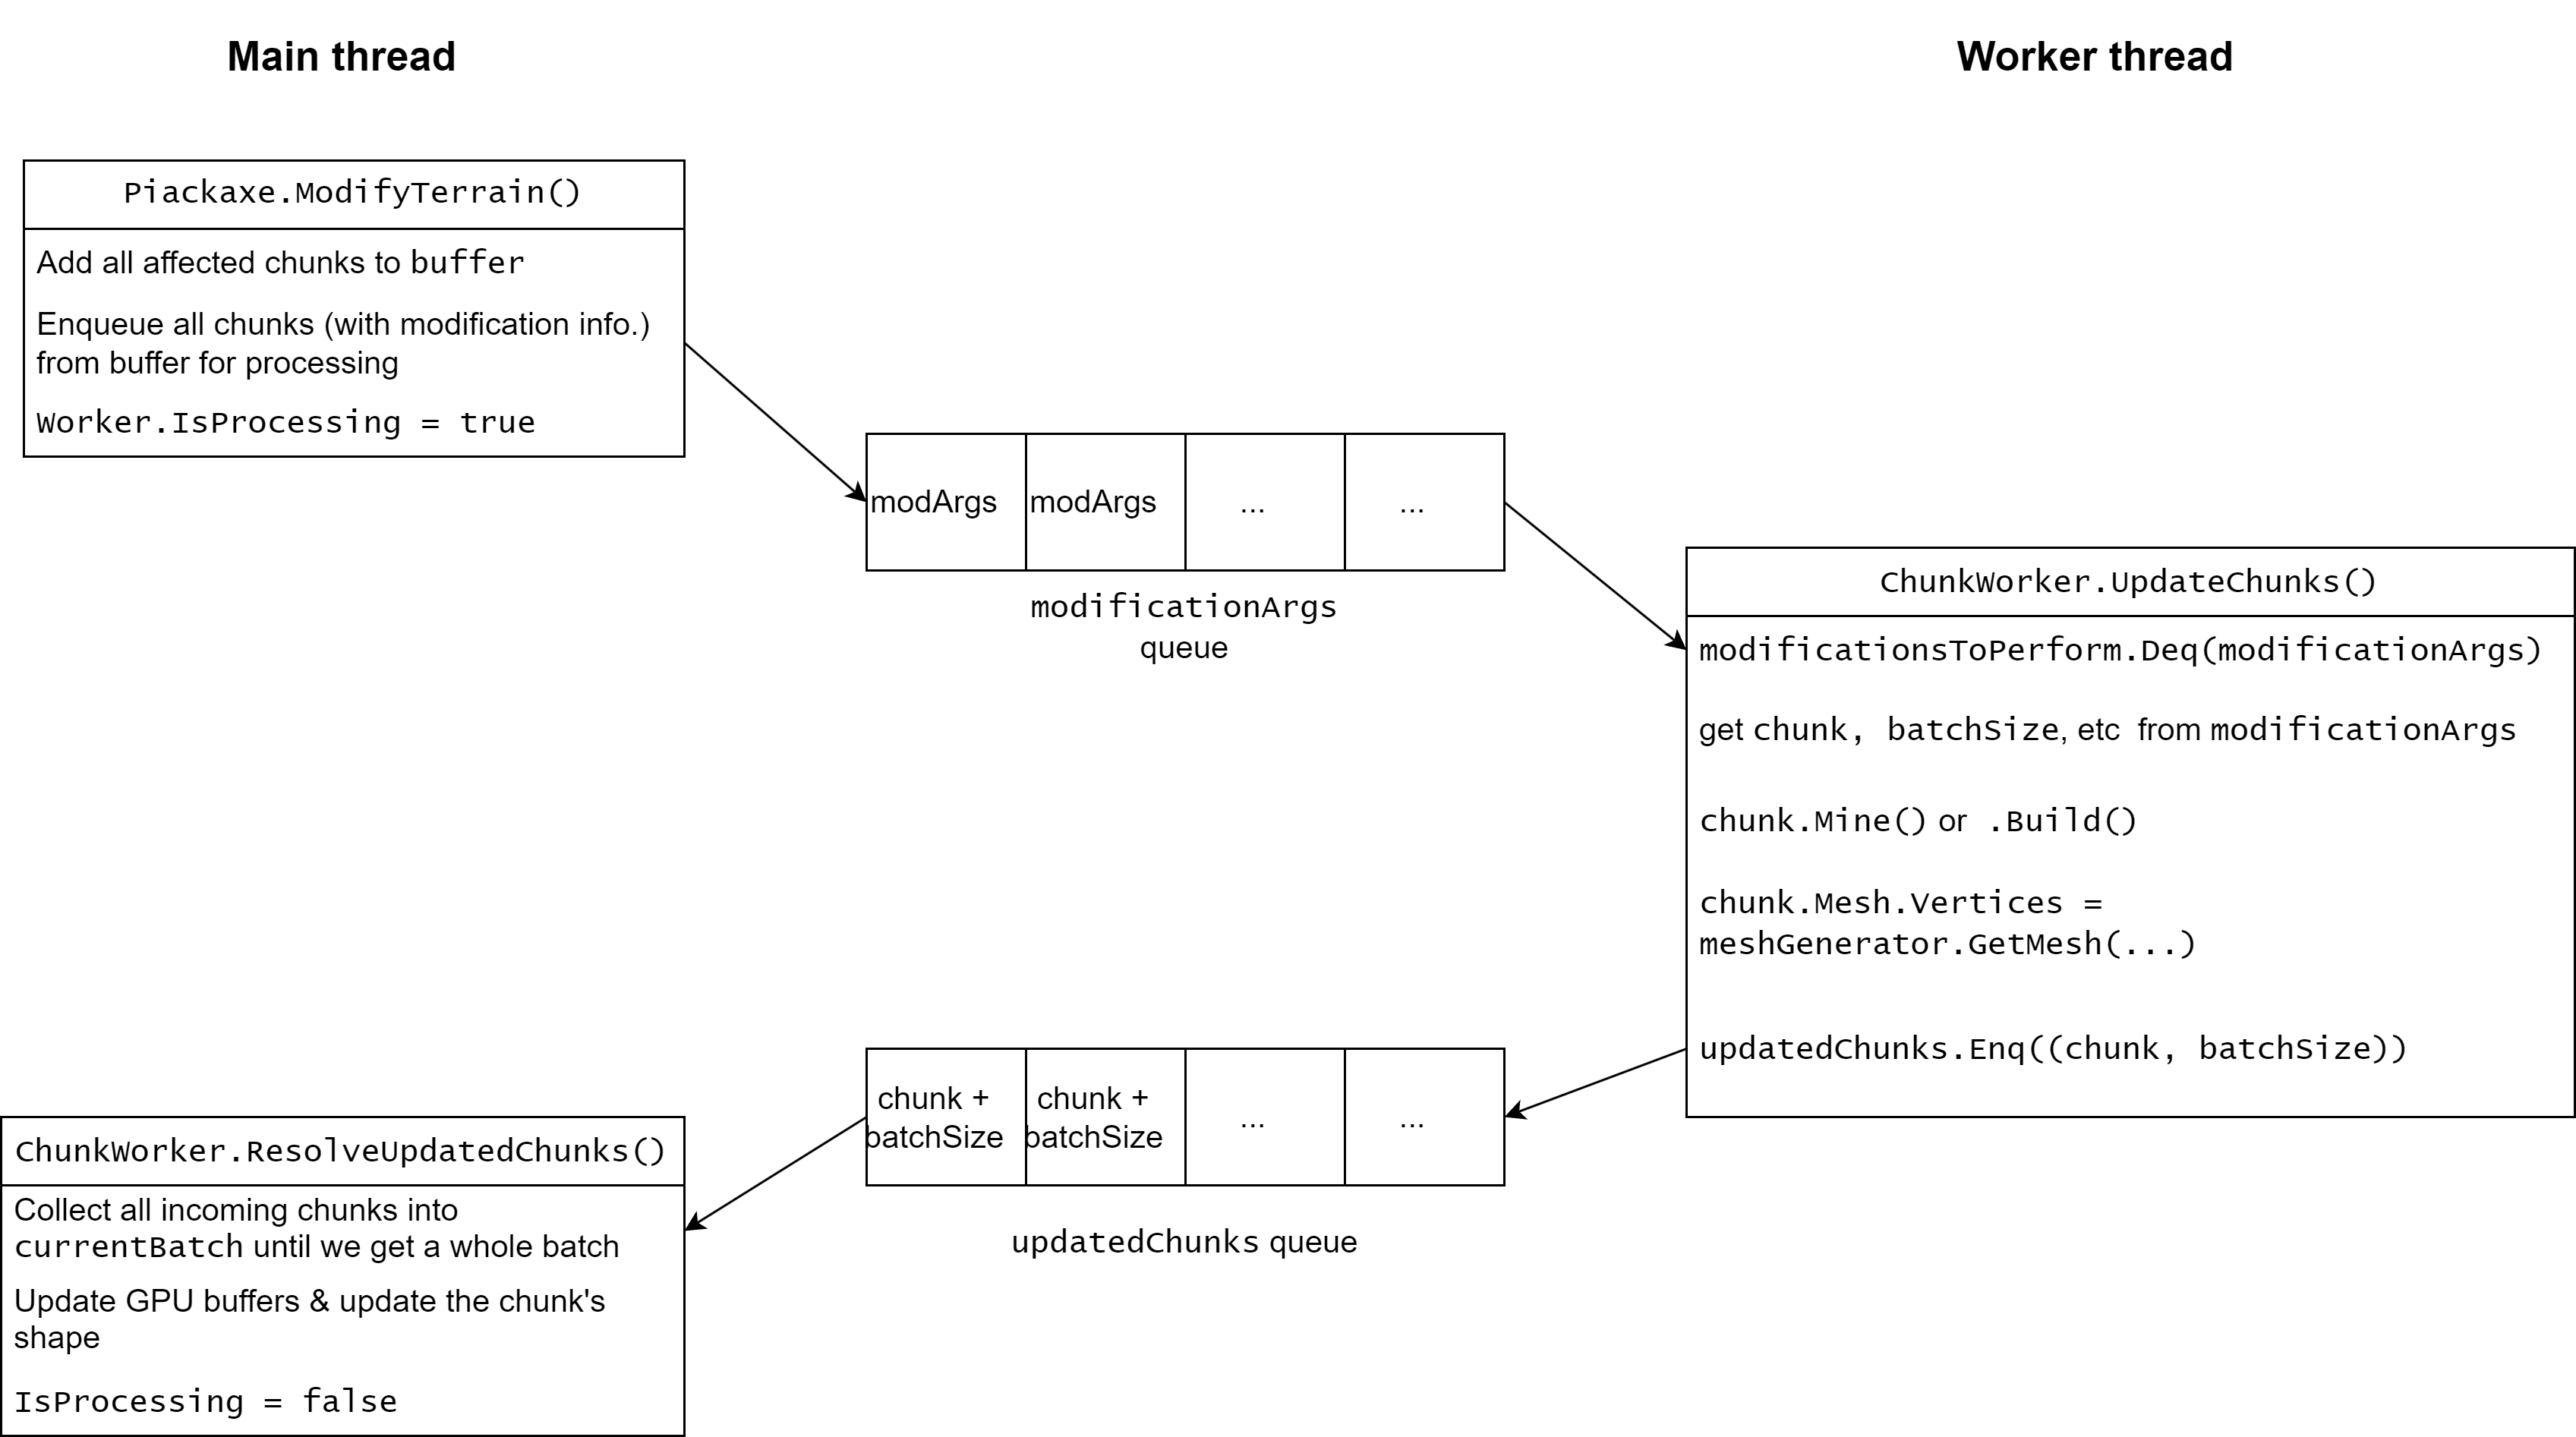
\includegraphics[width=1\textwidth]{chapters/implementation/sections/chunk_management_system/resources/chunkWorker.drawio.png}
    \caption{Terrain modification in the chunk management system}
    \label{fig:chunk-worker}
\end{figure}

The reason for processing chunks in batches rather than individually is simple.
If we modify chunks one by one it may be the case that when the terrain is rendered, one chunk has already been modified, while its neighbor has not, resulting in a visible gap between the two.
This problem can be seen in \autoref{fig:gaps-between-chunks-chunk-worker} which comes from an early stage of the game's development.
\begin{figure}[!htb]
    \centering
    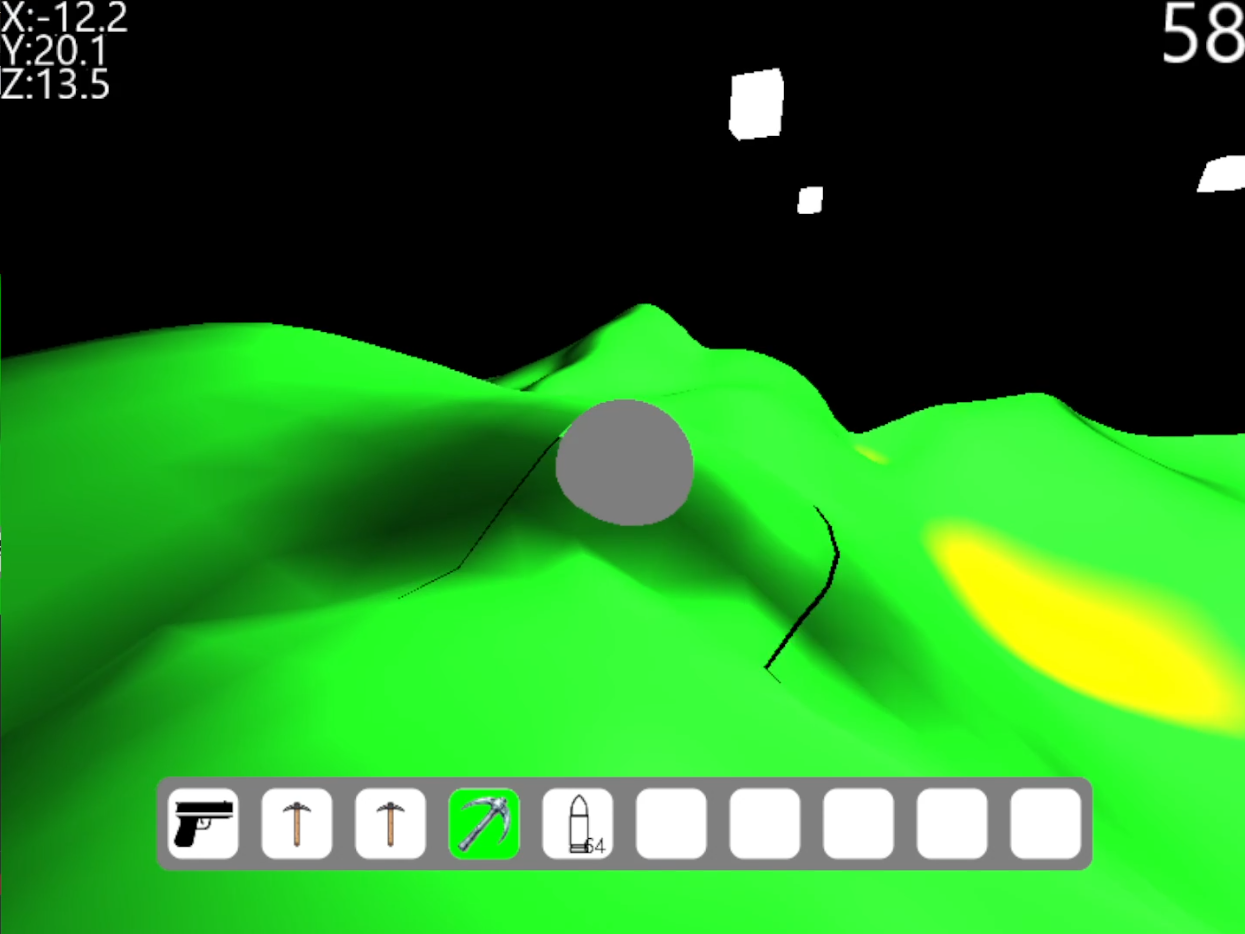
\includegraphics[width=0.6\textwidth]{chapters/implementation/sections/chunk_management_system/resources/gaps-between-chunks.png}
    \caption{Gaps between chunks appearing during terrain modification}
    \label{fig:gaps-between-chunks-chunk-worker}
\end{figure}

One drawback of this approach is that the main thread doesn't register new chunks for modification while the whole previously enqueued batch hasn't been processed.
This could cause the modification rate to be irregular should the main thread "drop" a lot of modifications.
To deal with this problem, the modification depends on the time elapsed between two modifications.